\documentclass{article}

\usepackage[utf8]{inputenc}
\usepackage{fancyhdr}
\usepackage{float}
\usepackage{tikz}
\usetikzlibrary{arrows}
\usetikzlibrary{positioning}
\pagestyle{fancy}

\renewcommand\thepart{\Alph{part}}

\title{Homework Module: A Controller for Swarm Behaviour in Webots}

\lhead{Homework Module \#1}
\rhead{IT3708 - Subsymbolic Methods in AI}
\cfoot{\thepage}

\author{
    Aleksander Burkow \\
    Sigve Sebstian Farstad \\
    Emil Grønnbeck
}

\begin{document}

\maketitle

\abstract{
This report presents a solution for Homework Module \#1 of IT3708, spring 2014 at NTNU.
The purpose of the homework module is to ``understand swarm behaviour by implementing a controller for box pushing task in Webots''.
}

\part{The Proposed System}

\section{Description}

\begin{figure}[H]
\centering
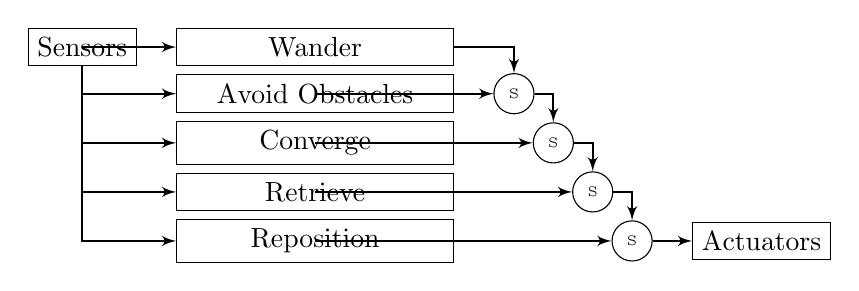
\begin{tikzpicture}

\tikzstyle{behaviour}=[draw, minimum width=10em, right=5mm of sensors]
\tikzstyle{line}=[draw, thick, -latex']
\tikzstyle{subsumption}=[draw, circle]

\node[draw] (sensors) {Sensors};

\node[behaviour] (wander) {Wander};
\node[behaviour, below=1mm of wander] (avoid_obstacles) {Avoid Obstacles};
\node[behaviour, below=1mm of avoid_obstacles] (converge) {Converge};
\node[behaviour, below=1mm of converge] (retrieve) {Retrieve};
\node[behaviour, below=1mm of retrieve] (reposition) {Reposition};

\node[subsumption, right=5mm of avoid_obstacles] (avoid_obstacles_subsumption) {\tiny S};
\node[subsumption, right=10mm of converge] (converge_subsumption) {\tiny S};
\node[subsumption, right=15mm of retrieve] (retrieve_subsumption) {\tiny S};
\node[subsumption, right=20mm of reposition] (reposition_subsumption) {\tiny S};
\node[draw, right=5mm of reposition_subsumption] (actuators) {Actuators};

\path[line] (sensors) |- (wander);
\path[line] (sensors) |- (avoid_obstacles);
\path[line] (sensors) |- (converge);
\path[line] (sensors) |- (retrieve);
\path[line] (sensors) |- (reposition);

\path[line] (avoid_obstacles) |- (avoid_obstacles_subsumption);
\path[line] (converge) |- (converge_subsumption);
\path[line] (retrieve) |- (retrieve_subsumption);
\path[line] (reposition) |- (reposition_subsumption);

\path[line] (wander) -| (avoid_obstacles_subsumption);
\path[line] (avoid_obstacles_subsumption) -| (converge_subsumption);
\path[line] (converge_subsumption) -| (retrieve_subsumption);
\path[line] (retrieve_subsumption) -| (reposition_subsumption);
\path[line] (reposition_subsumption) -- (actuators);

\end{tikzpicture}
\caption{The subsumption architecture of the proposed system.}
\label{figure:subsumption}
\end{figure}


\section{Simulation Results}

\part{An Improved System}

\section{Description}
\section{Simulation Results}

\part{A More Advanced Architecture}

\section{Description}
\section{Simulation Results}

\end{document}
